\documentclass[tikz,border=10pt]{standalone}
\begin{document}
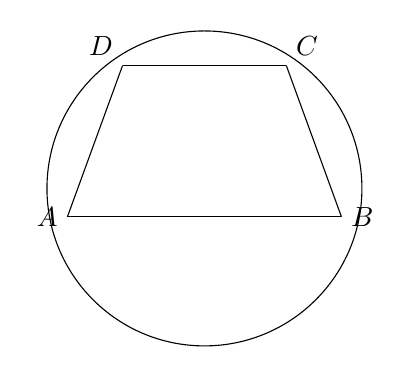
\begin{tikzpicture}[scale=2]
  % circle
  \draw (0,0) circle (1);
  % points
  \coordinate (A) at (-0.87,-0.18);
  \coordinate (B) at (0.87,-0.18);
  \coordinate (C) at (0.52,0.78);
  \coordinate (D) at (-0.52,0.78);
  % edges
  \draw (A) -- (B);
  \draw (B) -- (C);
  \draw (C) -- (D);
  \draw (D) -- (A);
  % labels
  \node[left] at (A) {$A$};
  \node[right] at (B) {$B$};
  \node[above right] at (C) {$C$};
  \node[above left] at (D) {$D$};
\end{tikzpicture}
\end{document}
